\section{A proof-of-concept example: \textnormal{\textit{learning acyclic stepping for locomotion}}}
\begin{figure}[t]
	\centering
	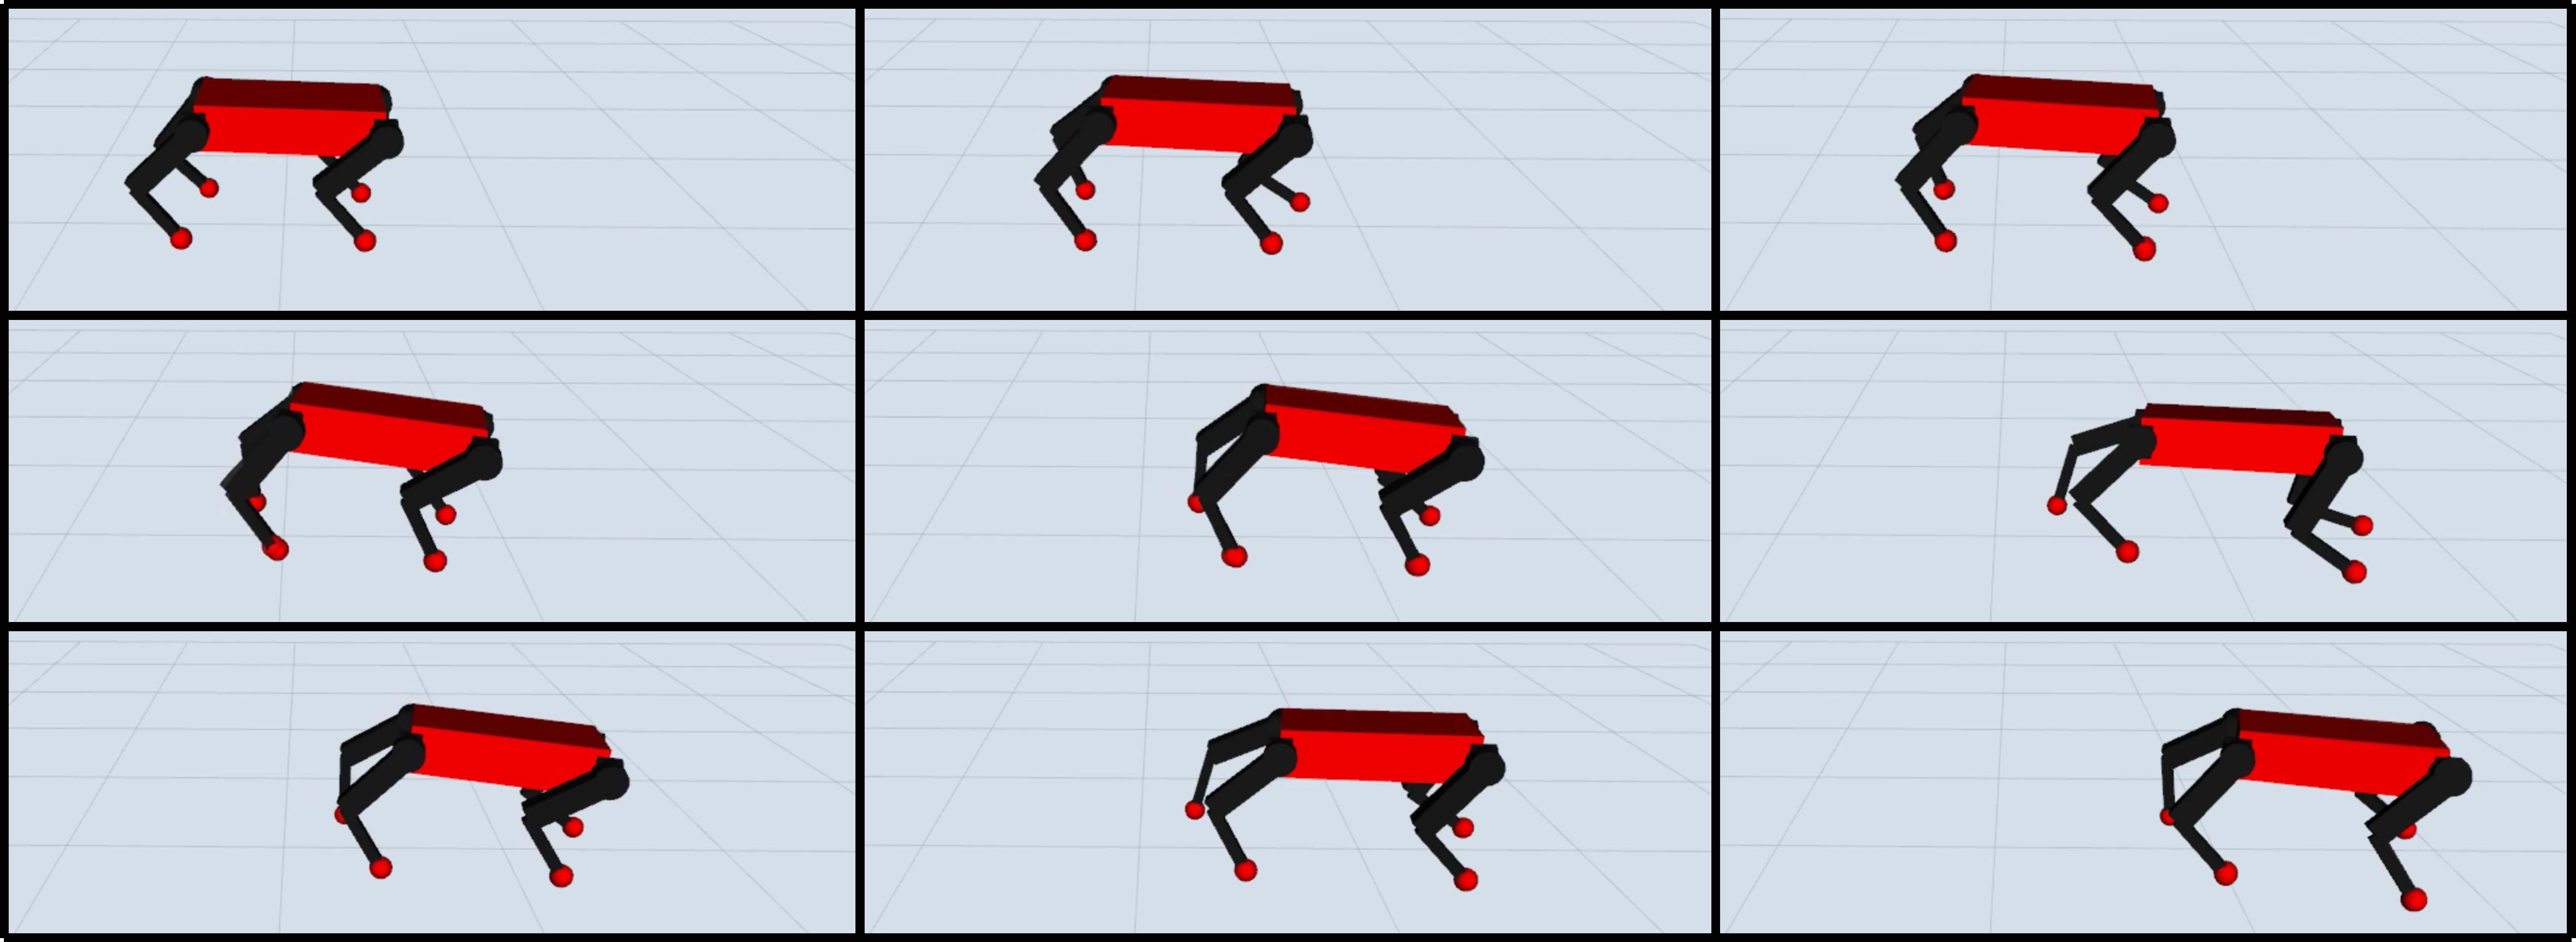
\includegraphics[width=0.9\columnwidth]{imgs/proof_of_concept.pdf}
	\caption{Preliminary results showing the agent during learning while it moves the robot forward using the RHC controller, from left to right and from top to bottom. The corresponding video is available at~\cite{web::poc_link}}
	\label{fig:proof}
\end{figure}
To showcase the potential of the proposed hybrid RL-RHC approach and of our framework, we trained a RL agent using PPO~\cite{rl:schulman2017proximal} to exploit a RHC controller for achieving a very simple forward locomotion task on a quadruped robot (shown in Fig.~\ref{fig:proof}). The agent is given a forward velocity reference and is continuously rewarded based on the task error and the performance of the underlying RHC controller. Notably, we observe the emergence of completely acyclic contact phases, varying from crawling to bound-like patterns.
 